\documentclass[12pt]{article}

\usepackage{graphicx,color}

\begin{document}

\title{Self-assembled soft solids in colloid-cholesteric mixtures}
\author{Ourselves \\ {\small Here and there}}
\date{}

\maketitle

{\bf Dispersion of particle inside liquid crystals have been shown to form new materials with tunable elastic and electrooptic properties~\cite{stark}. When the host is a blue phase~\cite{mermin}, a chiral liquid crystal with full three-dimensional periodicity, it has been proposed that the particles should self assemble into colloidal crystals which can selectively absorb light~\cite{miha,lavrentovich}. 
Here we present computer simulations which show that such colloid-cholesteric mixtures give actually rise to a much wider range of new soft solids than previously anticipated, encompassing regular crystals, glasses, cellular solids, isolated clusters, twisted rings and undulating colloidal ropes. The final self-assembled structure can be controlled by tuning the colloid concentration and the anchoring strength, that is the extent to which particles perturb the liquid crystalline alignment nearby. An important role is also played by the dynamical schedule with which colloids are introduced in the mixture, and by the ordering imparted through confining walls. The soft solids we find are metastable, and should be relevant to the design of new generation switchable multistable devices, which may be used to create, for instance, novel display and electronic paper technologies~\cite{epaper}.}

%Coles abstract/first paragraph:
%A promising approach to the fabrication of materials with
%nanoscale features is the transfer of liquid-crystalline structure
%to polymers1–11. However, this has not been achieved in systems
%with full three-dimensional periodicity. Here we demonstrate
%the fabrication of self-assembled three-dimensional nanostructures
%by polymer templating blue phase I, a chiral liquid
%crystal with cubic symmetry. Blue phase I was photopolymerized
%and the remaining liquid crystal removed to create
%a porous free-standing cast, which retains the chiral threedimensional
%structure of the blue phase, yet contains no chiral
%additive molecules. The cast may in turn be used as a hard template
%for the fabrication of new materials. By refilling the cast
%with an achiral nematic liquid crystal, we created templated
%blue phases that have unprecedented thermal stability in the
%range 􀀀125 to 125 C, and that act as both mirrorless lasers
%and switchable electro-optic devices. Blue-phase templated
%materials will facilitate advances in device architectures for
%photonics applications in particular.

%introduction on colloids in liquid crystals
%why it is interesting to consider a cholesteric liquid crystal or blue phase
%new materials: gels, photonic crystals and glasses

When spherical particles are mixed into a nematic liquid crystal, 
they disrupt the orientational order in the fluid and create defects,
or disclination lines, close to their surface. As these local drops in
the order increase the overall free energy of the system, it is advantageous
to gather many such deformations in one place, rather than distribute them 
uniformly in 3D throughout the fluid. Therefore these particles 
have a generic tendency to aggregate. Such aggregates may further 
self-assemble into lines~\cite{wiresmiha}, 2D crystals~\cite{zumer}, 
planar structures~\cite{tanaka}, or 3D amorphous glasses~\cite{tiffany}.
Besides being of fundamental interest to materials science, these
structures have tunable elastic and optical properties, hence 
they offer exciting prospects for applications as biosensors~\cite{abbott}, or
as new-generation display devices~\cite{colloiddevice}.

But one may also choose to disperse colloidal particles in a cholesteric, 
rather than nematic, liquid crystal. The molecules making up this material are
chiral, and this causes their average orientation to rotate in space in
a helical fashion, rather than stay constant as in nematics. 
This typically creates a 1-dimensional periodic structure whose wavelength 
is the pitch, $p$. The periodicity can however become 3D in the so-called 
blue phases (BPs). BPs arise because the molecule orientation -- the so-called 
director field -- can twist along more than one direction (see 
the cartoon in Fig. 1). Such double twist 
regions are energetically favoured due to the molecular chirality of the fluid,
however they lead to frustration because it is impossible to tile the whole 3D
space by putting together double twist regions without introducting
topological defects -- singularities where the director field is undefined.
These defects line up to form disclinations, which in blue phases may
either form 3D periodic regular crystals (the case of BPI and BPII) or be 
disordered, as in BPIII, aka the blue fog. BPs therefore are stabilised by
the tendency of chiral molecules to twist, and destabilised by the
elastic cost of forming topological defects and distorting the orientation.
This competition limited the temperature range in which they could be
observed in the past to a tiny neighbourhood or the order-disorder
transition. Current advances have increased the stability range by orders
of magnitude, up to an amazing 250 K, which has paved the road to
applications of BPs in display devices~\cite{kikuchi,coleswidetrange,bpdevice}.

%what is the use?? biosensors and photonic crystals then?? bistable
%devices? 

%why use cholesteric/blue phases? because they provide defect
%network even in the absence of particles!

Besides being remarkable materials {\it per se}, BPs make potentially
interesting hosts for dispersing colloidal particles as well. One reason
is that BPs form a disclination network even in the absence of
particles, so that they can potentially template their self-assembly. 
Indeed, as proved recently by simulations~\cite{miha}, one can imagine that 
when dispersing nanoparticles (which interact only weakly with the molecules
of a BP), such particles will be attracted to the defects in the BP
network. That is because, by covering up such disclinations, 
the system does not have to pay anymore the elastic cost associated with
defect formation, hence the free energy of the mixture decreases.
As the defect network is highly ordered in BPs, the particles will tend
to form a regular colloidal crystal, with the periodicity of BPs. 
Because, in turn, its associated wavelength lies in the visible range, 
the resulting material should have a photonic bandgap (albeit probably
an incomplete one, as the BPs themselves do~\cite{bplasers}), and can thus be used to 
control light propagation.
Another reason to study colloid-BP mixtures is that even in the absence
of particles there are several coexisting metastable minima in the system,
corresponding to different topologies of the defect network~\cite{adriano}. 
Adding particles
is likely to add more features in the free energy profiles, and if this
can be done in a controlled way the resulting system will be uniquely
placed to provide a bistable or multistable device, provided a strategy
can be found to kinetically access this or that minimum. Multistability
is highly sought after in new generation display devices, because it
endows samples with memory. For instance, a metastable state will not
change much even after the field which was needed to reach it is removed,
and this leads to huge saving in energy consumption. 

%what new here? phase transitions between different soft solids! tunability
%in the bulk: transition between photonic crystal, isolated clusters
%and self-quenched (blue phase) glass
%with confinement: transition between arrested loops, sheets 
%and cellular solids

We show in Fig. 2 results from large scale simulations which suggest the
existence of multiple phases for mixtures of colloidal particles 
(size $2R=100$ nm) of finite volume fraction in a BPI disclination network
(elastic constant $K= XXX$ pN, unit cell size XXX nm). 
We show in Fig. 1 the final states of four simulations (see Supporting 
Information for 
details) in which we first equilibrated 
a BPI network of disclination, for a choice of parameters (see Supporting
Information) 
for which such a state is the thermodynamically stable one, and then 
dispersed colloidal
particles, making up either 1\% (Fig. 2A and 2B) or 5\% (Fig. 2C and 2D)
of the total volume of the mixture. Briefly, our algorithm couples molecular
dynamics for the colloidal particles to continuum hydrodynamic theory
for the evolution of the tensorial order parameter of 
the blue phases (see Supporting Information). 
The liquid crystal director field tends
to align perpendicular to the surface of the colloidal particle, and
the strength of the anchoring is $W$. 

The value of the dimensionless ratio between the anchoring energy, $WR^2$, 
and the stored elastic energy due to the
nearby distortion in the ordering, $KR$, is well known to 
play an important role in the physics of a single colloidal particle
in a nematic fluid~\cite{stark}, where it controls the transition
between different topologies in the disclination accompanying the particle.
We find that this ratio, $WR/K$, is also a key contributor, together
with the colloidal volume fraction, to determine which soft solid assembles
starting from the random dispersion of particles in an ordered BP. 

%results from computer simulations in bulk cholesterics
%small anchoring particles go to defect lines
%large anchoring particles form either clusters or percolated networks 
%Fig. 1 on blue phases


When $WR/K$ is small (0.23 in Fig. 1A and 1C), the particles are
attracted to the disclination network, and cover up the defect lines
orderly to form a regular structure, similar to the photonic crystal
predicted in~\cite{miha}. Interestingly, the weak but finite anchoring
appears to lead to an elastic force between particles on a disclination lines
which sets a typical distance between them. In this
small $WR/K$ regime, it is the preexisting BP network which templates
the formation of a colloidal structure. It is likely that polymer-stabilised 
blue phases~\cite{kikuchi} 
work by a similar principle, based on a weak interaction between 
the monomers in the chain and the surrounding liquid crystal orientation. 

For $WR/K>1$ (see Fig. 2B and 2D), this picture changes dramatically.
In this case the colloidal particles disrupt significantly the
orientational order in the fluid, and this leads to the 
creation of new disclination close to their surface, similar 
to the Saturn rings which appear in nematics~\cite{stark}. The sharp drop in
liquid crystalline order within the BP leads now to a 
strong interparticle attraction, which restructures the disclination
network completely, such that the final result is quite distinct from
the original BPI topology. Most notably, the aggregates favour
the formation of defect junctions, where four disclinations meet
(similar to the structure of BPII rather than BPI). The 
particle clusters are disjoint for low volume fraction, but 
they interact elastically via the connecting disclinations.
As the volume fraction becomes larger, the aggregates join up
to form a percolating colloidal cluster which the BP disclinations
follow. All the structures in Fig. 1 should be soft solids, in
the sense that their zero-frequency elastic modulus, $G'$ should
be non-zero if probed via oscillatory rheology (unlike pure BPs where
$G'=0$ at zero frequency as the system can flow with a finite
viscosity via permeation~\cite{permeation1,permeation2}). We expect that the
structures in Fig. 1A-C should be weak gels, as here the 
defect network percolates but the particles do not, similarly
to what found in the cholesteric-nanoparticle gel stabilised
in~\cite{lubensky} (with $G'<1$ Pa). The ``cellular solid'' 
structure in Fig. 1D should be much more resistent mechanically, 
due to the formation of a thick percolating particle network. The 
structure is now akin to that of the self-quenched glass found in 
colloid-nematic composites~\cite{tiffany}, but for much higher volume 
fraction (over 20\% as opposed to below 5\% here). 

One may wonder how easy it is in practice to grow very regular blue
phase structures in the absence of colloidal nanoparticles. 
Before the technological advances of~\cite{kikuchi,coleswidetrange}
this was challenging and required fine tuning of temperature
and chirality: old experimental phase diagrams 
show that in a wider parameter range BPIII, which is amorphous, forms
in place of the ordered cubic BPI and BPII~\cite{mermin} (see 
typical experimental phase diagram in Fig. 1). 
Recent simulations also suggest that
domain growth in BPs favours disordered structures, and that the
nucleation of an ordered disclination crystal is probably hierarchical
and slow~\cite{domaingrowth,bp3}. 
What happens then when we disperse then colloids into a glassy
defect network, such as that of BPIII? Fig. 3 addresses this question,
for the same parameters used in Fig. 2. For small anchoring ($WR/K<1$),
the particles once again dress the disclination lines, but this time they
give rise to a glassy structure rather than to a crystal, as such
is the nature of the underlying network which acts as a template.
Increasing the volume fraction again leads to a more even coverage with
a rather well defined particle spacing (compare Fig. 3A and 3B). 
For large anchoring ($WR/K>1$), on the other hand, the pattern is very
much alike that seen in Fig. 1: now it is the particles which dictate
the self-assembly, and we observe isolated clusters at low volume 
fraction, and cellular solids for higher colloid concentration
(see Fig. 3C and 3D). As expected, the free energy of the soft solids
obtained by dispersing nanoparticles inside these disordered networks
is considerably higher than the one found with the stable regular BPI
structure (see Supporting Information, Fig. S1). 
Nevertheless, all these structures
are metastable, as the elastic forces keeping them together dwarf thermal
energy from Brownian motion (see the scales of energies and energy
differences in Fig. S1).

%sandwiches: effect of anchoring on the structure of the soft solid
%soft solid: G'\ne 0 

The existence of several locally stable competing solids with 
very different symmetry and, arguably, physical properties, 
is of interest to technology, as it makes these materials ideal
candidate to build multistable devices, which can retain memory of
more than one metastable state in the absence of an applied field.
Multistability is indeed a must-have feature for new generation switchable 
electrooptic devices for use in energy-saving electronics-free
appliances, smart glass, and e-paper to cite just a few examples.
However, state-of-the-art liquid crystal display devices are
rarely so large that the bulk description in Fig. 2 and 3 is relevant to
them. Typically, the fluid is strongly confined in these devices, and the
boundary effects cannot be disregarded. Therefore in what follows we describe
how colloidal suspensions self assemble in thin sandwiches, where
the confining walls are treated so as to favour planar or 
perpendicular (homeotropic) anchoring of the liquid crystal.

Fig. 4 shows the case of normal anchoring at the wall, again for
small (Fig. 4A and 4C) and large (Fig. 4B and 4D) values of
$WR/K$. Initially the liquid crystal is quenched from the isotropic
to the ordered phase as done for Fig. 3, for similar parameter values 
as previously used. Therefore, a metastable glassy disclination network
arises once again (see Supplementary Material): the conflict between the
normal anchoring at the wall and the tendency of the liquid crystal to
twist in the bulk further hinders the formation of a regular structure.
The structures formed by dispersing nanoparticles within this network
are somewhat similar to the ones already observed in the bulk: at low
values of $WR/K$ the particles simply hop on the network (Fig. 4A and 4C), 
whereas for large anchoring at the colloid surface we observe isolated
clusters (Fig. 4B) and percolated cellular solids (Fig. 4D), for
``small'' (1\%) and ``large'' (5\%) particle volume fraction respectively.
There are however important differences, due to the key role played
by the boundaries. 
First, the normal anchoring at the wall recruits particles there,
so that the colloids aggregate either on the planes or towards the middle of
the sample (see the side view of the snapshots in Fig. 4). Second,
the clusters formed for strong anchoring (see Fig. 4D in particular) 
are planar, similarly to those observed in
colloid-cholesteric mixtures for large particle
size~\cite{niek}.
 
The case of planar wall anchoring is treated in Fig. 5 and leads to
striking differences, and yet more self-assembled structures. 
Without colloids, the planar anchoring now leads to
the formation of a regular cholesteric helix,
with axis perpendicular to the boundary walls. 
This twisted texture forms by annealing away an initial loop defect network,
which shrink and disappear to leave a defect-free sample. However,
dispersing particles with small $WR/K$ arrests the loop shrinking process,
and particles stabilise twisted figure-of-eight rings for dilute
suspensions, or plectonemic structures for more concentrated ones (see Fig. 5A
and 5C respectively). 
For larger $WR/K$, structures form thick fibers, with diameter about
5-fold larger than that of single colloids (see Fig. 5B and 5D). 
These colloidal ropes are undulating due to the chiral structure of the 
underlying fluid, and develop branching points upon increasing the particle
density, to eventually converge again into cellular solids once the suspension
becomes concentrated enough. The wall-induced ordering now is incompatible
with the homeotropic anchoring at the colloid surface, and particle
are this time repelled from the wall (see the side views of the
configurations in Fig. 5).

%Conclusions

The surprising wealth of structures obtained in Figs. 2-5 is the complex 
consequence of a simple competition between two self-assembly principles. 
First, blue phases and cholesteric defect networks provide a three-dimensional 
template of disclinations to which colloidal particles are attracted, in order 
to lower the free energy of the mixture. Second, colloidal intrusions in a 
liquid crystal lower the orientational order locally, hence are subjected to a 
generic tendency to aggregate into clusters to minimise such elastic
distortions. Which of these principles dominates depends on the value of a key 
dimensionless parameter in the system, $WR/K$, which measures the strength of 
the anchoring of the liquid crystal director field at the colloidal surface. 
If this ratio is low, the templating principle dominates: according to
the wall coating and the initial disclination network chosen (BPI or BPIII) 
we get colloidal crystals, glasses or twisted rings. If $WR/K$ is high,
flocculation wins over templating, and we end up with isolated aggregates,
percolating cellular solids, or helical colloidal ropes according to
boundary properties and the volume fraction of the dispersion. All these
soft solids will have different, and tunable, elastic and optical properties,
hence are highly promising for the design of future multistable liquid
crystal devices, which are at the forefront of current technological 
developments in this field.

\begin{thebibliography}{99}
\bibitem{stark} H. Stark, {\it Phys. Rep.} {\bf 351}, 387-474 (2001).
\bibitem{mermin} Wright D.~C., Mermin, N.~D. Crystalline liquids: The blue phases. {\it Rev. Mod. Phys.} {\bf 61}, 385–432 (1989).
\bibitem{miha} M. Ravnik, G.~P. Alexander, J.~M. Yeomans,  
S. Zumer, {\it Proc. Natl. Acad. Sci. USA} {\bf 108}, 5188-5192 (2011).
\bibitem{lavrentovich} O.~D. Lavrentovich, {\it Proc. Natl. Acad. Sci.
USA} {\bf 108}, 5143-5144 (2011).
\bibitem{epaper} J. Heikenfeld, P. Drzaic,  J.~S. Yeo, T. Koch.
A critical review of the present and future prospects for electronic paper.
{\it J. Soc. Inf. Display} {\bf 19}, 129-156 (2011).
\bibitem{zumer} I. Musevic, M. Skarabot, U. Tkalec, M. Ravnik,
S. Zumer, {\it Science} {\bf 313}, 954-958 (2006).
\bibitem{tiffany} T.~A. Wood, J.~S. Lintuvuori, A.~B. Schofield, D. Marenduzzo,
W.~C.~K. Poon, {\it Science} {\bf 333}, 79-83 (2011).
\bibitem{abbott} I.~H. Lin, D.~S. Miller, P.~J. Bertics, C.~J. Murphy, J.~J. de Pablo, N.~L. Abbott, {\it Science} {\bf 332}, 1297-1300 (2011).
\bibitem{colloiddevice} K. Chari, C. M. Rankin, D. M. Johnson, T. N. Blanton,
R. G. Capurso. Single-substrate cholesteric liquid crystal displays by colloidal self-assembly. {\it Appl. Phys. Lett.} {\bf 88}, 043502 (2006).
\bibitem{crooker} D. K. Yang and P. P. Crooker, {\it Phys. Rev. A}
{\bf 35}, 4419 (1987).
\bibitem{kikuchi} H. Kikuchi, M. Yokota, Y. Hisakado, H. Yang, T. Kajiyama.
Polymer-stabilized liquid crystal blue phases.
{\it Nat. Mat.} {\bf 1}, 64-68 (2002).
\bibitem{coleswidetrange} H.~J. Coles, M.~N. Pivnenko.
Liquid crystal 'blue phases' with a wide temperature range.
{\it Nature} {\bf 436}, 997-1000 (2005).
\bibitem{bpdevice} Z.~B. Ge, S. Gauza, M.~Z. Jiao, H.~Q. Xianyu, S.~T. Wu,
{\it Appl. Phys. Lett.} {\bf 94}, 101104 (2009).
\bibitem{bplasers} W. Y. Cao, A. Munoz, P. Palffy-Muhoray, B. Taheri.
Lasing in a three-dimensional photonic crystal of the liquid crystal blue 
phase II. {\it Nat. Mat.} {\bf 1}, 111-113 (2002).
\bibitem{permeation1} 	W. Helfrich. Capillary flow of cholesteric
and smectic liquid crystals. {\it Phys. Rev. Lett.} {\bf 23}, 372-374 (1969).
\bibitem{permeation2} A. Dupuis, D. Marenduzz, E. Orlandini, J.~M. Yeomans.
Rheology of cholesteric blue phases. {\it Phys. Rev. Lett.} {\bf 95},
097801 (2005).
\bibitem{lubensky} M. Zapotocky, L. Ramos, P. Poulin, T.~C. Lubensky, 
D.~A. Weitz, {\it Science} {\bf 283}, 209-212 (1999).
\bibitem{coles} F. Castles, F.~V. Day, S.~M. Morris, D-H. Ko, D.~J. Gardiner, M.~M. Qasim, S. Nosheen, P.~J.~W. Hands, S.~S. Choi, R.~H. Friend, H.~J. Coles, {\it Nat. Mat.} {\bf 11}, 599-603 (2012).
\bibitem{domaingrowth} O. Henrich, K. Stratford, D. Marenduzzo, M.~E. Cates,
{\it Proc. Natl. Acad. Sci. USA} {\bf 107}, 13212-13215 (2010).
\bibitem{bp3} O. Henrich, K. Stratford, M.~E. Cates, D. Marenduzzo,
{\it Phys. Rev. Lett.} {\bf 106}, 107802 (2011).
\bibitem{wiresmiha} M. Ravnik, M. Skarabot, S. Zumer, U. Tkalec, I. Poberaj, D. Babic, N. Osterman, I. Musevic, {\it Phys. Rev. Lett.} {\bf 99}, 247801 (2007).
\bibitem{tanaka} T. Araki, H. Tanaka, {\it Phys. Rev. Lett.} {\bf 97}, 
127801 (2006).
\bibitem{tanakanatmat} T. Araki, M. Buscaglia, T. Bellini, H. Tanaka,
{\it Nat. Mat.} {\bf 10}, 303-309 (2011).
\bibitem{adriano} A. Tiribocchi, G. Gonnella, D. Marenduzzo, E. Orlandini,
F. Salvadore, {\it Phys. Rev. Lett.} {\bf 107}, 237803 (2011).
\bibitem{fukuda} J.-I. Fukuda, S. Zumer, {\it Nat. Comm.} {\bf 2}, 246 (2011).
\bibitem{niek} Hijnen N., Wood T.~A., Wilson D., Clegg P.~S. 
Self-Organization of Particles with Planar Surface Anchoring in a Cholesteric
 Liquid Crystal. {\it Langmuir} {\bf 26}, 13502-13510 (2010).
\end{thebibliography}

\newpage

\begin{figure}
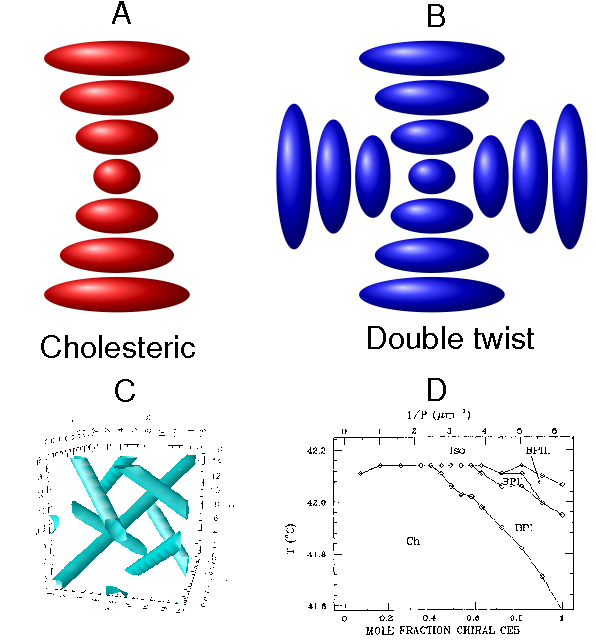
\includegraphics[width=\textwidth]{s0.png}
\caption{Schematics of the molecular arrangement in a 
cholesteric helix (A) and within a double twist cylinder (B, the
axis of the cylinder is perpendicular to the plane of the page).
The disclinations line arrangement in the unit cell of BPI is shown in
(C), while a reference phase diagram (from Ref.~\cite{crooker}) is
shown in (D).}
\end{figure}

\begin{figure}
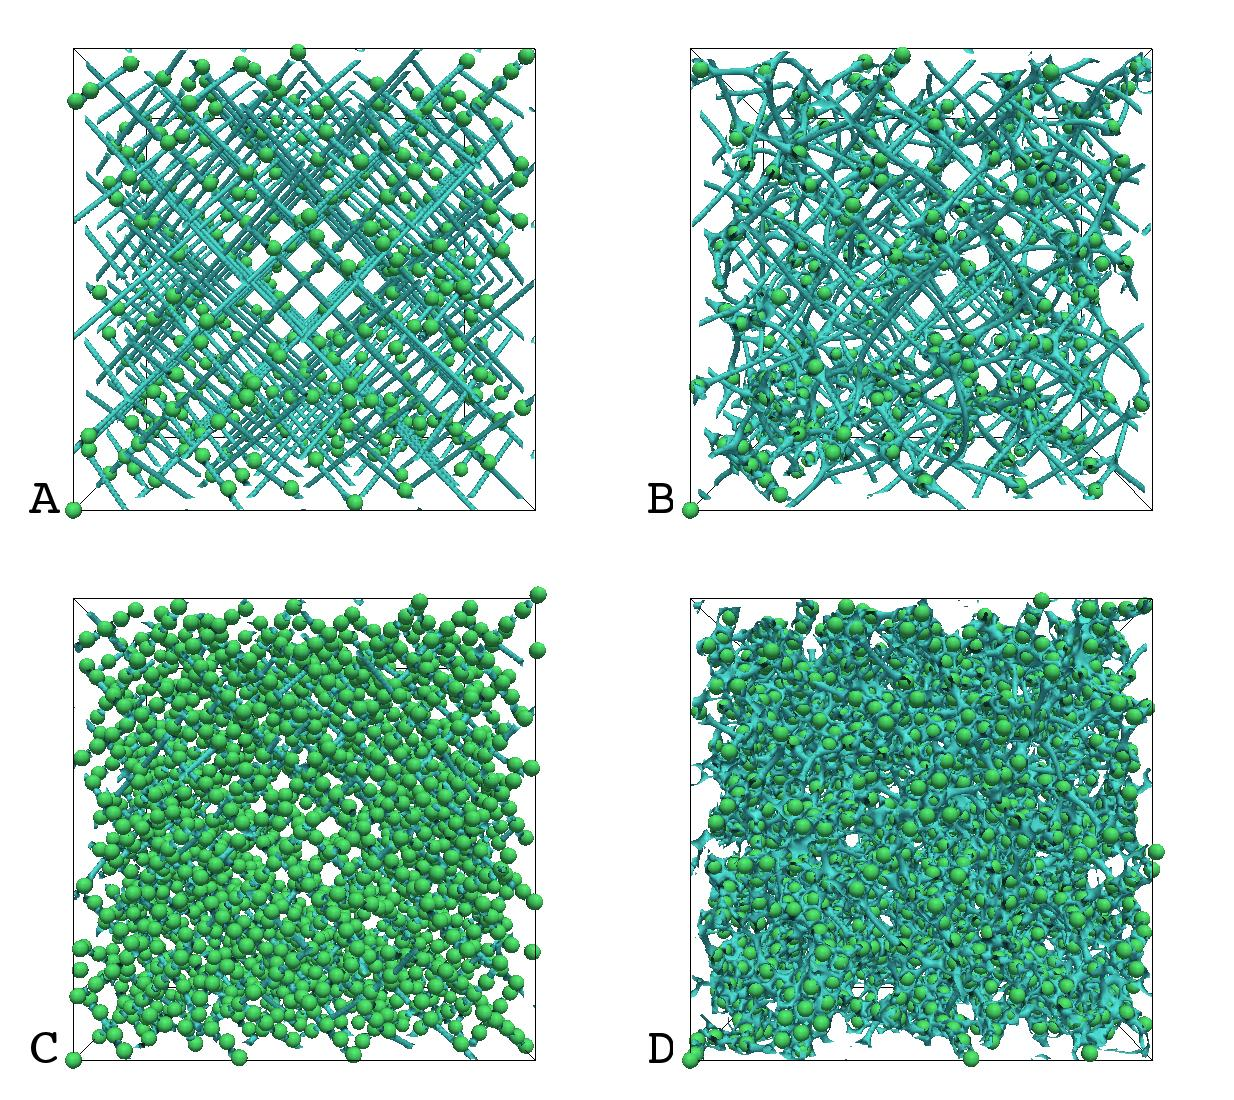
\includegraphics[width=\textwidth]{s1.jpg}
\caption{Snapshots of the steady states obtained after dispersing
a suspension of colloidal nanoparticles inside blue phase I, initially
in its thermodynamic equilibrium structure. Structures correspond
to (A) $WR/K=0.23$ and $\phi=1\%$, (B) $WR/K=2.3$ and $\phi=1\%$,
(C) $WR/K=0.23$ and $\phi=5\%$, (D) $WR/K=2.3$ and $\phi=5\%$.
The anchoring of the director field to the colloidal surface is normal.
[For the full parameter list used to generate Figs. 2-5, 
in simulation units, see Supporting Information.] }
\end{figure}

\begin{figure}
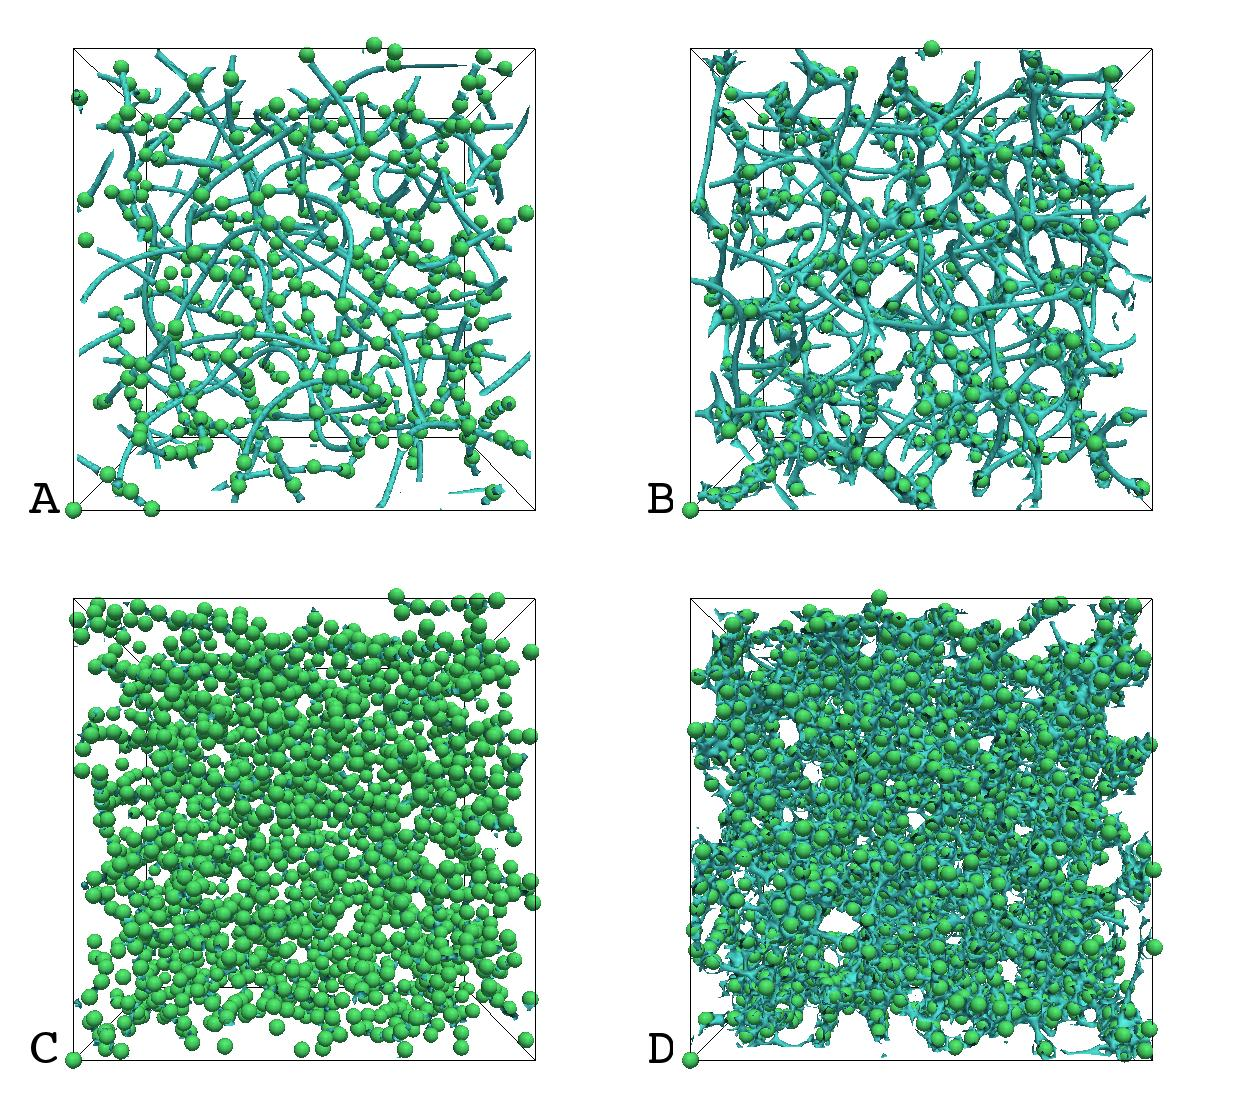
\includegraphics[width=\textwidth]{s2.jpg}
\caption{Same as Fig. 2, but now the disclination network
inside which the nanoparticles are dispersed is 
amorphous, and we prepared it through
a quench from the isotropic into the blue phase  I region.}
\end{figure}

\begin{figure}
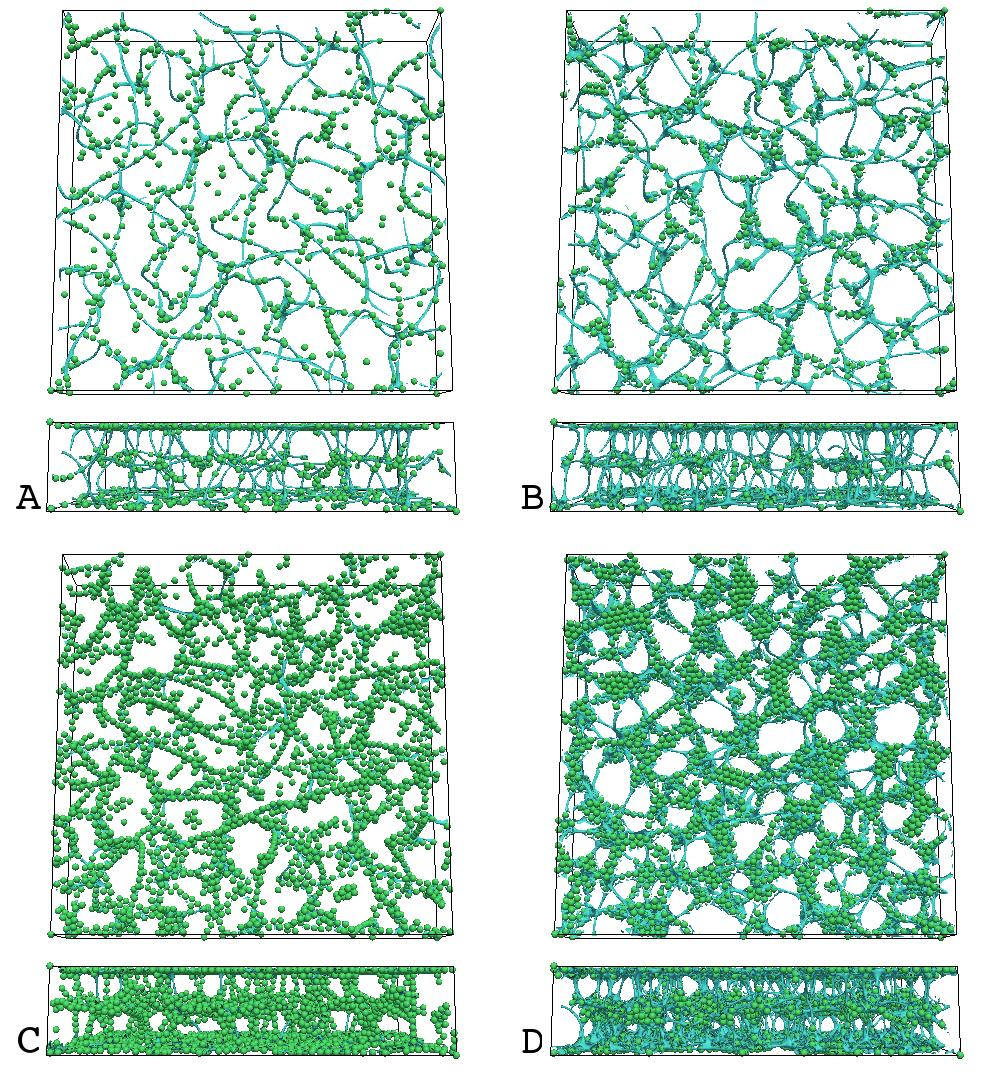
\includegraphics[width=\textwidth]{s3.jpg}
\caption{Snapshots of the steady states obtained after dispersing
a suspension of colloidal nanoparticles inside a sandwich filled with
cholesteric liquid crystal, with normal anchoring of the director field
at the boundaries. Both top and side views are provided. 
Structures correspond
to (A) $WR/K=XXX$ and $\phi=1\%$, (B) $WR/K=XXX$ and $\phi=1\%$,
(C) $WR/K=XXX$ and $\phi=2\%$, (D) $WR/K=XXX$ and $\phi=2\%$.
}
\end{figure}

\begin{figure}
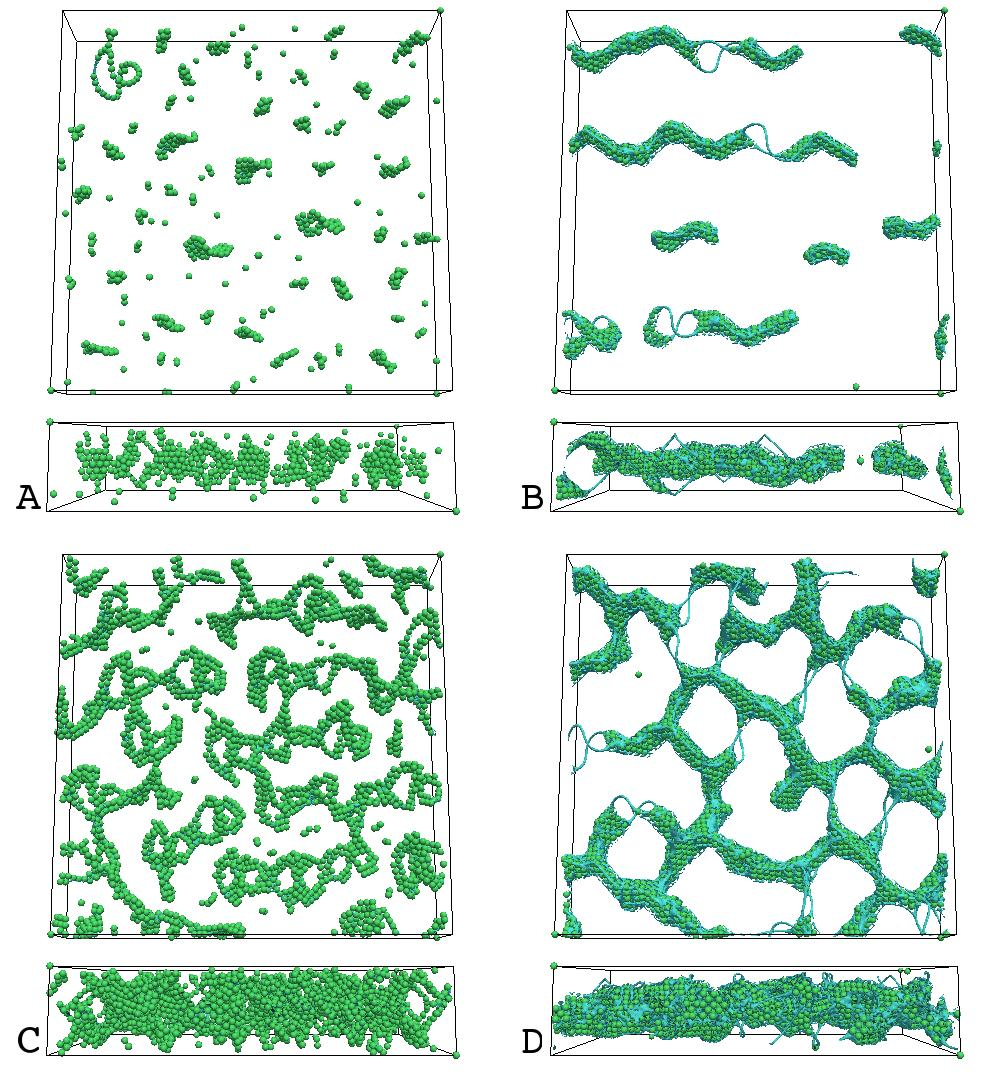
\includegraphics[width=\textwidth]{s4.jpg}
\caption{Same as Fig. 4, but with planar anchoring of the director 
field to the boundary planes.}
\end{figure}

\end{document}
